\documentclass[xcolor=table]{beamer}

\usepackage{shyne}

% Theme settings
\setbeamertemplate{navigation symbols}{}

\usetheme{Madrid}
\usefonttheme{structurebold}

\AtBeginSection[]
{ 	\begin{frame}{}

	{
	\usebeamerfont{frametitle}
	\begin{beamercolorbox}
		[wd={\textwidth}, center, sep=.2in, rounded=true, shadow=true]
		{frametitle}
	Chapter \thesection\\  \secname 
	\end{beamercolorbox}
	}
	
	\end{frame} 
}

\AtBeginSubsection[]
{ 	\begin{frame}{}

	{
	\usebeamerfont{frametitle}
	\begin{beamercolorbox}
		[wd={\textwidth}, center, sep=.2in, rounded=true, shadow=true]
		{frametitle}
	Section \thesection .\thesubsection\\  \subsecname 
	\end{beamercolorbox}
	}
	
	\end{frame} 
}

\title[Chapter 1]{Stat 201: Statistics I\\ Chapter 1 }
\author[M. Shyne]{}
\institute[Metro State]{
\includegraphics[width=1.75in]{../images/metro_logo}}
\date[Jan 8, 2018]{January 8, 2017
\\ \bigskip \bigskip 
\includegraphics[width=.4in]{../images/cc_big}}


\begin{document}

\frame{\titlepage}

% Chapter 1
\section{Introduction to Statistics}

% Section 1.1
\subsection{Statistical and Critical Thinking}

\begin{frame}{What is statistics?}
\begin{block}{}
\large
``Statistics is the language of science."
\end{block}

\pause
\begin{block}{}
Statistics is also the language of...
\begin{itemize}
\item Politics (both campaigns and public policy)
\item Economics
\item Business
\item Psychology and social sciences
\item \ldots
\end{itemize}

\end{block}
\end{frame}

\begin{frame}{What is statisitcs?}

\begin{block}{}
\large \bt{Statistics} is the science of using data to learn about the world.
\end{block}

\pause
\begin{block}{}
\large \bt{Data} are collections of observations, such as measurements, biographical information or survey responses.
\end{block}

\pause
\begin{block}{}
Statistics is involved in\ldots
\begin{itemize}
\item Designing studies and experiments
\item Collecting data
\item Producing informative summaries of data
\item Analyzing data
\item Interpreting results (answering questions)
\end{itemize}
\end{block}

\end{frame}

\begin{frame}{Populations and samples}

\begin{block}{}
\large A \bt{population} is any group that we are interested in knowing something about.
\end{block}

\pause
\begin{block}{}
\large A \bt{census} is when data is collected from \emph{every} member of a population.
\end{block}

\pause
\begin{block}{}
\large A \bt{sample} is a subset of a population used to represent the whole population.
\end{block}

\end{frame}


\begin{frame}{Population and sample examples}

\begin{exampleblock}{Example}
\begin{center}
\begin{tabular}{p{1.8in} | p{1.8in} }
Population & Sample\\
\hline
The entire population of the United States & Respondents to an internet survey\pause\\ 
Males over 40 who have high blood pressure & High blood pressure patients in a clinical trial\pause\\

Students enrolled at Metro State in 2017 & You (the students in this class)\pause\\
Statistics classes in Minnesota & The summer semester statistics classes at Metro State\\
\end{tabular}
\end{center}
\end{exampleblock}

\end{frame}


\begin{frame}{Statistical thinking}

\begin{block}{Prepare}
\begin{itemize}
\item [1] Context
\item [2] Source of the data
\item [3] Sampling method
\end{itemize}
\end{block}

\begin{block}{Analyze}
\begin{itemize}
\item [1] Graph the data
\item [2] Explore the data
\item [3] Apply statistical method
\end{itemize}
\end{block}

\begin{block}{Conclude}
\begin{itemize}
\item [1] Significance
\end{itemize}
\end{block}

\end{frame}

\begin{frame}
\frametitle{Prepare: Context}
\begin{block}{}
\begin{itemize}
\item What do the data mean?
\item What is the goal of the study?
\item Can the data answer the question of interest?
\end{itemize}
\end{block}

\pause
\begin{exampleblock}{Example}
Suppose a group of researchers wants to study the association between intelligence and grades. So, they collect the GPAs of a random sample of students and measure their skull circumference\ldots\\
\end{exampleblock}
\pause
\begin{alertblock}{Note}
This is not a completely made up example. Phrenology was the study of skull sizes and shapes, and was used as recently as the early 20th century to ``prove" that non-white races were inferior and to diagnose mental illness.
\end{alertblock}
\end{frame}

\begin{frame}
\frametitle{Prepare: Source of the data}
 
\begin{block}{}
\begin{itemize}
\item Are the data from a source with a special interest so that there is pressure to obtain results that are favorable to the source?
\end{itemize} 
\end{block}

\pause
\begin{exampleblock}{Example}
According to an article in the NY Daily News from June, 2014, titled, ``Strip down: Sleeping naked is good for your relationship, survey says" (\href{http://www.nydailynews.com/life-style/health/survey-sleeping-naked-good-relationships-article-1.1849491}{link)}\ldots\\
\medskip
From a survey of 1000 British couples, ``57\% of those who reported sleeping in the buff said they felt happy, compared with 48\% of pajama wearers and 43\% of nightie wearers."\\

\begin{itemize}
\pause\item The survey was conducted by Cotton USA.
\end{itemize}
\end{exampleblock}

\end{frame}

\begin{frame}
\frametitle{Prepare: Sampling method}
 
\begin{block}{}
\begin{itemize}
\item Were the data collected in a way that is biased?
\end{itemize} 
\end{block}
 
\pause
\begin{block}{}
\large A \bt{voluntary response sample} (or \bt{self-selected sample}) is one in which the respondents themselves decide whether to be included. 
\end{block}

\pause
\begin{exampleblock}{Example}
\begin{itemize}
\item Call-in polls to radio or tv stations\ldots
\pause\item Online surveys\ldots
\pause\item Trending on twitter\ldots
\end{itemize}
\end{exampleblock}
\end{frame}

\begin{frame}
\frametitle{Analyze}
 
\begin{block}{}
\begin{itemize}
\item [1] Graph the data
\item [2] Explore the data
\begin{itemize}
\item Are there any outliers?
\item What important statistics summarize the data?
\item How are the data distributed?
\item Are there missing data?
\end{itemize}
\item [3] Apply statistical method
\end{itemize}
\end{block}

\begin{block}{}
Most of the course concerns the analyze step.
\end{block}
\end{frame}

\begin{frame}
\frametitle{Conclude: Significance}

\begin{block}{}
\begin{itemize}
\item Do the results have statistical significance?
\begin{itemize}
\item Statistical significance is a measure of how unlikely observed results are given certain assumptions.
\item Statistical significance is determined by many factors, including study design.
\end{itemize}
\item Do the results have practical significance?
\begin{itemize}
\item Do the results matter?
\end{itemize}
\end{itemize}
\end{block}

\pause
\begin{exampleblock}{Example}
A clinical trial shows a new drug lowers systolic blood pressure by an average of 3 mmHg. Results might be statistically significant, but are probably not practically significant.
\end{exampleblock}
\end{frame}

\begin{frame}
\frametitle{Potential pitfalls: Misleading conclusions}

\begin{block}{}
Mistaking an association or relationship between two variables or factors for one factor causing the other.
\end{block}

\pause

\begin{alertblock}{!!!}
\Large Correlation does not imply causation.
\end{alertblock}

\pause
\begin{exampleblock}{Example}
Recall the sleeping naked study.\\
\medskip
Though the article made the claim that sleeping naked \bt{caused} happier relationships, the study merely pointed to an association.\\
\medskip
There are many other possible explanations for that association. This study alone does not provide evidence for which explanation is ``true".

\end{exampleblock}

\end{frame}

\begin{frame}
\frametitle{Other potential pitfalls}

\begin{block}{}
\begin{itemize}
\item \bt{Reported results} are data provided by the subjects of a study, rather than measured directly.
\pause\item \bt{Sample size} is important. Be wary of results drawn from very small samples.
\pause\item \bt{Loaded questions} are those designed to elicit a particular response or to influence the subject.
\begin{itemize}
\item Also known as: push polls
\end{itemize}
\pause\item The \bt{order of questions} can influence responses.
\pause\item \bt{Missing data} can introduce bias if there are characteristics shared by subjects who have missing data or those who do not.
\end{itemize}
\end{block}


\end{frame}


\begin{frame}
\frametitle{Potential pitfalls: Precise numbers}

\begin{block}{}
Precision is not the same thing as accuracy.
\end{block}

\begin{center}
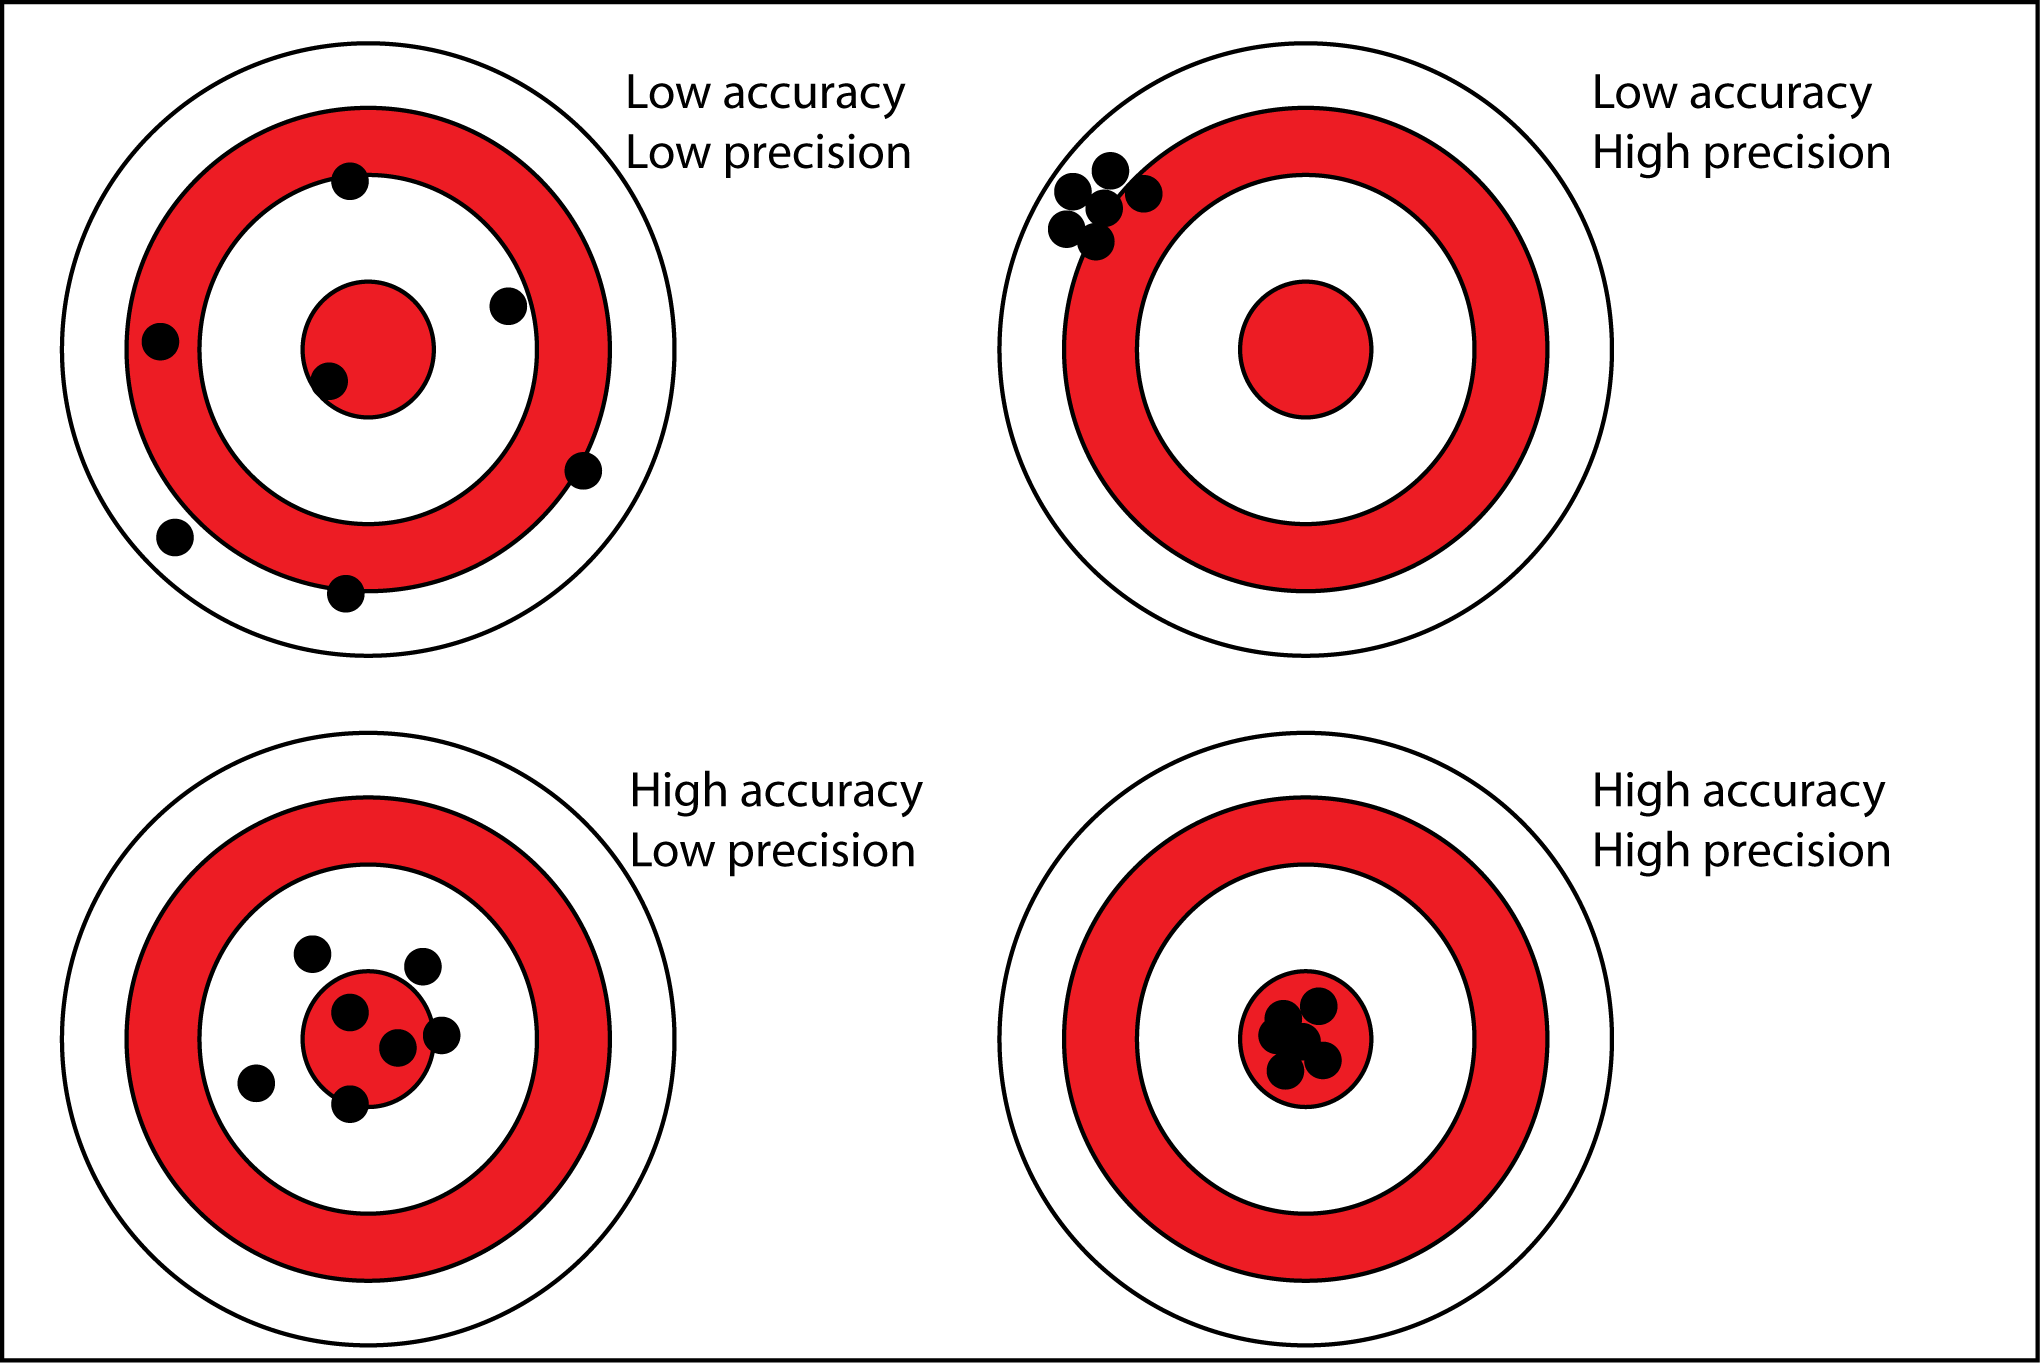
\includegraphics[width=3.5in]{../images/precision_accuracy}
\end{center}
\end{frame}

\begin{frame}
\frametitle{Potential pitfalls: Percentages}

\begin{block}{}
Sometimes percentages are used in confusing ways. Remember, 100\% of a thing is all of it. Percentages above 100, or phrases like ``a reduction of 100\%", do not always have clear meanings. 
\end{block}


\end{frame}

\begin{frame}
\frametitle{Percentages: Review}

\begin{block}{}
\begin{itemize}
\item A \bt{percentage} is number describing a proportion as an amount out of 100 (per cent).
\pause
\item We can also describe a \bt{proportion} as a fraction of 1.
\[\ds \frac {50}{100} = \frac 1 2 \quad \implies \quad 50\% = .50\]
\pause
\item 100\% represents a whole, just as for proportions 1 represents a whole.
\pause
\item It often doesn't make sense to talk about percentages greater than 100\%.
\end{itemize}
\end{block}
\end{frame}

\begin{frame}
\frametitle{Percentages: Calculations}
\begin{exampleblock}{}
To convert from percentage to proportion, divide by 100:
\[56\% \quad \implies \quad \frac {56}{100} = 0.56\]

To convert from proportion to percentage, multiply by 100:
\[\frac 5 8 = 0.625 \quad \implies \quad 0.625 \times 100 = 62.5\%\]

To find the quantity a percentage represents:
\[\text{13\% of 264}\quad \implies \quad \frac {13}{100} \times 264 = 34.32\]

To find the percentage a quantity represents:
\[\text{135 out of 475} \quad \implies \quad \frac {135}{475} \times 100 = 28.42\ldots \%\]
\end{exampleblock}
\end{frame}

\begin{frame}<handout:0>{Group work}
\begin{block}{}
\large
\begin{itemize}
\item Get into groups of 2 - 4
\item Introduce yourself. Tell your groups your major and why you are taking this class. 
\item For each question, read the scenario. Discuss and note some answers to part (a).
\item Don't worry about getting exactly the right answers. Thinking about and discussing the question is more important.
\item After about 15 minutes we will discuss as a class. 
\end{itemize}
\end{block}
\end{frame}



% Section 1.2
\subsection{Types of Data}

\begin{frame}
\frametitle{Parameters and statistics}

\begin{block}{}
\large A \bt{parameter} is a value describing an aspect of a population.
\end{block}
\pause
\begin{block}{}
\large A \bt{statistic} is a value describing an aspect of a sample.
\end{block}
\pause
\begin{exampleblock}{Example}
\begin{itemize}
\item The average height of adult men in the U.S. is 72 inches: \bt{Parameter}

\item The average height of 30 randomly selected male Metro State students is 68.5 inches: \bt{Statistic}
\end{itemize}
\end{exampleblock}

\end{frame}

\begin{frame}
\frametitle{Types of data}

\begin{block}{}
\large \bt{Quantitative} data are numbers representing amounts, sizes, time or other measurements.\\
Also known as: Numeric
\end{block}

\begin{exampleblock}{Example}
Class size, height, age, systolic blood pressure, temperature
\end{exampleblock}

\pause

\begin{block}{}
\large \bt{Categorical} data are values representing groups or categories.
\begin{itemize}
\item Also known as: qualitative, attribute
\end{itemize}
\end{block}

\begin{exampleblock}{Example}
Gender, state of residence, football player's numbers, pain scale
\end{exampleblock}

\end{frame}

\begin{frame}{Types of data: Quantitative}
\begin{block}{}
\large \bt{Discrete} data have a finite, or countably infinite, number of possible values. There are gaps in the possible values.
\end{block}

\begin{exampleblock}{Example}
Class size: can't have a class size of 22.5
\end{exampleblock}
\pause
\begin{block}{}
\large \bt{Continuous} data have an infinite number of possible values. There are no gaps in possible values.
\end{block}

\begin{exampleblock}{Example}
Height: a height of 70.2641... inches is possible (not necessarily useful, but possible)
\end{exampleblock}

\end{frame}

\begin{frame}{Levels of measurement}
\begin{block}{}
\large
\begin{itemize}
\item Nominal
\item Ordinal
\item Interval
\item Ratio
\end{itemize}
\end{block}
\end{frame}


\begin{frame}{Levels of measurement: Nominal}
\begin{block}{}
\large The \bt{nominal} level of measurement is categorical data that are names or labels for groups or categories. There is no reasonable order or ranking to the categories.
\end{block}
\pause
\begin{exampleblock}{Example}
\begin{itemize}
\item Gender: \emph{male} or \emph{female}
\item State of residence: \emph{Minnesota}, \emph{Wisconsin}, etc.
\end{itemize}
\end{exampleblock}
\pause
\begin{alertblock}{Hint}
The root word \emph{nom} means ``name''.
\end{alertblock}
\end{frame}

\begin{frame}
\frametitle{Levels of measurement: Ordinal}
\begin{block}{}
\large
The \bt{ordinal} level of measure is categorical data that are naturally ordered or ranked.
\end{block}
\pause
\begin{exampleblock}{Example}
\begin{itemize}
\item Pain scale: \emph{No pain} $<$ \emph{Moderate pain} $<$ \emph{Heavy pain}
\item Grades: \emph A $>$ \emph B $>$ \emph C $>$ \emph D $>$ \emph F
\end{itemize}
\end{exampleblock}
\end{frame}

\begin{frame}
\frametitle{Levels of measurement: Interval}
\begin{block}{}
\large The \bt{interval} level of measurement is quantitative data where\\ the difference between values has meaning but where there is no natural ``zero''.
\end{block}
\pause
\begin{exampleblock}{Example}
\begin{itemize}
\item Temperature: The difference between 101\textdegree F and 98.6\textdegree F is meaningful, but 0\textdegree F does not mean no temperature.
\item Year: 2017 is four years after 2013, but year 0 does not mean no years.
\end{itemize}
\end{exampleblock}
\end{frame}

\begin{frame}
\frametitle{Levels of measurement: Ratio}
\begin{block}{}
\large The \bt{ratio} level of measurement is quantitative data where the difference between values and relative sizes of values have meaning. There is a natural ``zero''.
\end{block}
\pause
\begin{exampleblock}{Example}
\begin{itemize}
\item Age: Someone who is 40 years old is \emph{twice} as old as someone who is 20 years old. Zero does mean no age.

\item Height: A tree that is 10 feet tall is \emph{one third} as tall as a tree that is 30 feet tall. Zero does mean no height.
\end{itemize}

\end{exampleblock}
\end{frame}

\begin{frame}<handout:0>{Group work}
\begin{block}{}
\large
\begin{itemize}
\item Get back into your groups.
\item Discuss and note some answers to part (b) for each question.
\item Remember, getting exactly the right answer is less important than the discussion.
\item After about 15 minutes we will discuss as a class. 
\end{itemize}
\end{block}
\end{frame}

%%%%
% 	Section 1.3
%%%%
\subsection{Collecting Sample Data}

\begin{frame}
\frametitle{Samples}

\begin{block}{}
\begin{itemize}
\large
\item Recall, when we want to know something about a population and we can't collect data from the entire population, we can collect data from a subset, or a \bt{sample}, of the population instead.
\pause
\item We can then use statistics to learn something about the whole population.
\pause
\item Therefore, how we pick our sample is very important in how valid the interpretation of our results are.
\end{itemize}
\end{block}
\pause
\begin{exampleblock}{Example}
\begin{itemize}
\item Suppose an organization is interesting in the taco consumption by Metro State students. It would be difficult, if not impossible, to ask every student about their taco eating habits. A sample is needed.
\end{itemize}
\end{exampleblock}
\end{frame}

\begin{frame}
\frametitle{Types of samples: Random sample}

\begin{block}{}
\large A \bt{random sample} is a sample selected such that every individual member of a population has an equal chance of being included.
\end{block}
\pause
\begin{block}{}
\large A \bt{simple random sample} is a sample selected such that every possible sample of a specific size has an equal chance of being selected.
\begin{itemize}
\item These are the ``best" kind of samples for producing valid, unbiased results, but they are not always easy to get. 
\end{itemize}
\end{block}
\pause
\begin{exampleblock}{Example}
\begin{itemize}
\item Given an alphabetical list of students, use a random number generator to select a sample.
\end{itemize}
\end{exampleblock}

\end{frame}

\begin{frame}
\frametitle{Types of samples: Systematic sampling}

\begin{block}{}
\large \bt{Systematic sampling} is a method where every $k$th member of of a population is selected.
\begin{itemize}
\item These samples are ofter easier to produce, but can lead to biased samples. 
\end{itemize}
\end{block}
\pause
\begin{exampleblock}{Example}
\begin{itemize}
\item Given an alphabetical list of students, select every fifth student until you have a sample of the desired size.
\end{itemize}
\end{exampleblock}

\end{frame}

\begin{frame}
\frametitle{Types of samples: Convenience sampling}

\begin{block}{}
\large \bt{Convenience sampling} is a method of choosing members of a population that are nearby or easy to access.
\begin{itemize}
\item The easiest of all methods, but by far the lowest quality data for producing results.
\end{itemize}
\end{block}
\pause
\begin{exampleblock}{Example}
\begin{itemize}
\item Wander the halls before class, asking students who happen to walk by.
\item Put a poll on the Metro State website.
\end{itemize}

\end{exampleblock}
\end{frame}

\begin{frame}
\frametitle{Types of samples: Stratified sampling}

\begin{block}{}
\large \bt{Stratified sampling} is a method where the population is divided into groups and samples are selected from each group.
\begin{itemize}
\item Useful when you want to ensure that a factor of interest has enough representation, but it is not a random sample as we have defined it.
\end{itemize}
\end{block}
\pause
\begin{exampleblock}{Example}
\begin{itemize}
\item If we have particular interest in the taco consuming difference between graduate students and undergrads, select a sample from each group.
\end{itemize}
\end{exampleblock}
\end{frame}

\begin{frame}
\frametitle{Types of samples: Cluster sampling}

\begin{block}{}
\large \bt{Cluster sampling} is a method where the population is divided into sections or clusters. Then, a number of clusters are randomly selected and all members of the clusters are included in the sample.
\begin{itemize}
\item More convenient than some methods, but better randomization the pure convenience sampling.
\end{itemize}
\end{block}
\pause
\begin{exampleblock}{Example}
\begin{itemize}
\item Choose 5 random classes, and survey all the students in those classes.
\end{itemize}
\end{exampleblock}
\end{frame}

\begin{frame}
\frametitle{Types of samples: Multistage sampling}

\begin{block}{}
\large \bt{Multistage sampling} is a when a combination of methods are used to produce a sample.
\end{block}
\pause
\begin{exampleblock}{Example}
\begin{itemize}
\item Choose random classes by cluster sampling, and then take a simple random sample of students from each chosen class.  
\end{itemize}
\end{exampleblock}
\end{frame}

\begin{frame}
\frametitle{Types of studies}

\begin{block}{}
\large In an \bt{observational study} data is collected from a sample without trying to modify behavior or results. 
\end{block}
\pause
\begin{block}{}
\large In an \bt{experiment} a change (treatment) is made to some or all of sample and then data is collected in order to detect changes. 
\end{block}

\end{frame}

\begin{frame}{Types of observational studies}

\begin{block}{}
\large
A \bt{cross-sectional} study measures and collects data from one point in time (the present).
\end{block}
\pause
\begin{block}{}
\large
A \bt{retrospective} study collects data from the past, whether from recollections or by examining records.
\begin{itemize}
\item Also know as: case-control
\end{itemize}
\end{block}
\pause
\begin{block}{}
\large
A \bt{prospective} study follows subjects into the future to measure and collect data.
\begin{itemize}
\item Also know as: longitudinal study, cohort study
\end{itemize}
\end{block}
\end{frame}

\begin{frame}{Experiment design: Replication}
\begin{block}{}
\large
\bt{Replication} is the repetition of the experiment on more than one individual or in more than one study.

\begin{itemize}
\pause\item Experimental studies should have adequate sample sizes to ensure that observed effects are ``true" effects and not due to individual characteristics or chance.
\pause\item Experimental studies should be, but rarely are, repeated by different researchers to verify results.
\end{itemize}
\end{block}
\end{frame}

\begin{frame}{Experimental design: Blinding}
\begin{block}{}
\large
\bt{Blinding} is the process of hiding which treatment or lack of treatment a subject is receiving from one or more groups of study participants. This is done in order to reduce bias in the results.

\begin{itemize}
\pause\item A \bt{single blinded} study is one where the subjects don't know what treatments they are receiving.

\pause\item A \bt{double blinded} study is one where both the subjects and the researchers administrating treatment and gathering results don't know which treatment the subjects are receiving.
\end{itemize}
\end{block}

\pause
\begin{block}{}
\large
The \bt{placebo effect} is a phenomenon where people who believe they are being treated demonstrate improvement.
\end{block}
\end{frame}

\begin{frame}{Experimental design: Randomization}

\begin{block}{}
\large
\bt{Randomization} is the process selecting samples and assigning treatment groups randomly. This is done to ensure that samples are representative of populations and that characteristics are evenly distributed among treatment groups.
\end{block}

\pause
\begin{block}{}
\large
\bt{Confounding variables} (or just confounders) are unmeasured and possible unknown factors that affect the experimental outcome. 
\end{block}
\end{frame}

\begin{frame}<handout:0>{Group work}
\begin{block}{}
\large
\begin{itemize}
\item Get back into your groups.
\item Discuss and note some answers to part (c) for each question.
\item After about 10 minutes we will discuss as a class. 
\end{itemize}
\end{block}
\end{frame}

\end{document}